\documentclass[dvipdfmx,autodetect-engine,10pt,b5paper,papersize,openany,dvipsnames]{jsbook}


\usepackage{color}
\usepackage{titlesec}
\usepackage{multicol}

% 本文をゴシックに
\usepackage[deluxe]{otf}
\renewcommand{\kanjifamilydefault}{\gtdefault}
\renewcommand{\familydefault}{\sfdefault}

\usepackage{amsmath,txfonts}
\usepackage{bm}
\usepackage{mathrsfs} % \mathscr

\usepackage[dvipdfmx]{graphicx}

% PDF を読み込み
\usepackage{pdfpages}

\usepackage{fancyhdr}

\usepackage{tikzpagenodes}
%\usepackage[object=vectorian]{pgfornament}
\usetikzlibrary{shapes.geometric,calc}


% AddToShipoutPictureBG*
\usepackage{eso-pic}


%\usepackage[dvipdfmx]{hyperref}
\usepackage[hidelinks]{hyperref}
\usepackage{pxjahyper}


\usepackage{listings}
\lstset{
  title={},
  caption={},
  frame={single},
  numbers=none,
  lineskip=-0.5ex,
  basicstyle={\small\ttfamily},
  identifierstyle={\small},
  commentstyle={\smallitshape},
  keywordstyle={\small\bfseries},
  ndkeywordstyle={\small},
  stringstyle={\small\ttfamily},
}

% https://oku.edu.mie-u.ac.jp/~okumura/jsclasses/
% jsbook の余白が広すぎます
% 書籍では1行の長さが全角40文字を超えないようにしています。
% そのため,段組をしないときは,自動的にどちらかの余白が広くなります
% (美文書シリーズのようなデザインになります)。
% これが困るときはプリアンブル(\begin{document} の前)に次のように書いてください。
\setlength{\textwidth}{\fullwidth}
\setlength{\evensidemargin}{\oddsidemargin}

% for \ruby{}{}
\usepackage{okumacro}

% 奥付
\newcommand{\bhline}[1]{\noalign{\hrule height #1}}

\title{
  \textbf{月刊 ZENKEI AI MAGAZINE\\
  2021年3月号}
}
\author{\textbf{\textsf{ZENKEI AI FORUM}}}
\date{}

\pagestyle{fancy}
\fancyhf{} % 既定設定をリセット
\renewcommand{\headrulewidth}{0pt} % 罫線無し
\fancyfoot[C]{\thepage}

\AtBeginDocument{
  \addtocontents{toc}{\protect\thispagestyle{fancy}}
}

\begin{document}

%\maketitle


\thispagestyle{fancy}
\setcounter{page}{1}
\AddToShipoutPictureBG*{%
  \AtPageLowerLeft{%
    \includegraphics[width=\paperwidth,height=\paperheight]%
      {images/MET-57007_r.jpg}
  }%
}%

\tableofcontents

\begin{tikzpicture}[remember picture,overlay]
\node[yshift=-9em,yscale=1.2,xslant=0.25,color=Gray] (text)
  at (current page.north){%
  \sffamily \large
  【月刊 ZENKEI AI MAGAZINE 2021年3月号】};
\end{tikzpicture}

\vspace{3cm}

\hfill
\begin{minipage}{0.45\textwidth}
{\small
    \noindent
    \textgt{\bfseries \sffamily 使用図版}\\
    メトロポリタン美術館に収蔵のデジタル化され\\
    パブリックドメインで公開されている\\
    \textmc{\bfseries 葛飾北斎}の
    \textmc{\bfseries 冨嶽三十六景}から
}
\end{minipage}

\vspace{1em}

{\small
  \begin{itemize}
    \setlength{\leftskip}{7.5cm}
  \item 表紙裏、ページ 1 : \textmc{\bfseries 凱風快晴}
    (\href{https://www.metmuseum.org/art/collection/search/57007}{MET-57007})
  \item ページ 2 -- 3 : \textmc{\bfseries 甲州石班沢}
    (\href{https://www.metmuseum.org/art/collection/search/39656}{MET-39656})
  \item ページ 30 -- 31 : \textmc{\bfseries 神奈川沖浪裏}
    (\href{https://www.metmuseum.org/art/collection/search/45434}{MET-45434})
  \item ページ 32、裏表紙裏 : \textmc{\bfseries 山下白雨}
    (\href{https://www.metmuseum.org/art/collection/search/57006}{MET-57006})
  \end{itemize}
}

\newpage

\AddToShipoutPictureBG*{%
  \AtPageLowerLeft{%
    \includegraphics[width=\paperwidth,height=\paperheight]%
      {images/MET-39656_l_mask.jpg}
  }%
}%

\chapter*{まえがき}
\addcontentsline{toc}{chapter}{まえがき}
\thispagestyle{fancy}
\begin{tikzpicture}[
  remember picture, overlay]
\node[yshift=-8em,yscale=1.2,xslant=0.25,color=Gray] (text)
  at (current page.north){%
  \sffamily \large
  【月刊 ZENKEI AI MAGAZINE 2021年3月号】};
\end{tikzpicture}

早いもので、2021年1月からスタートした ZENKEI AI MAGAZINE (ZAM) も
この2021年3月号で3冊目になります。

そろそろ軌道に乗ってきたか?と聞かれると、はい、とは言い切れませんね。
今回は ZENKEI AI FORUM の重要なコンセプトの1つである
diversity を象徴する、ゲスト・スピーカーによる寄稿が2編あります。

お楽しみください。

\begin{flushright}
  2021年5月25日\\
  金沢にて\\
  ZENKEI AI MAGAZINE 編集長\\
  市來健吾
\end{flushright}

\begin{tikzpicture}[remember picture, overlay]
  \begin{scope}[thick,rounded corners=8pt,
      line width=16pt,
      xscale=1.3, yscale=1.3, xshift=-1.75cm, yshift=-5.0cm]
  \draw (0, 2) -- (5, 2) -- (4, 0) [sharp corners] -- (5.5, 0)
    [rounded corners=8pt] -- (6.5, 2) [sharp corners] -- (7.5, 0)
    -- (8.5, 0);
  \draw (3.5, 0.8) -- (7.5, 0.8)
    -- (8.2, 2) -- (9.2, 0) -- (10.2, 2) -- (10.2, 0) -- (14, 0);
  \end{scope}
\end{tikzpicture}


\newpage

\AddToShipoutPictureBG*{%
  \AtPageLowerLeft{%
    \includegraphics[width=\paperwidth,height=\paperheight]%
      {images/MET-39656_r_mask.jpg}
  }%
}%

\chapter{当日のイベントの模様}
\label{sec:introduction}
\thispagestyle{fancy}

3月の ZAF はゲストをお二方、
通称「チーム・ホンダ」から
リーダーのホンダナオさんと、
チームの右腕の大島圭祐さんをお迎えして、
昨年2020年8月の ZAF で発表してもらった『東海道5X』の
その後の発展について発表していただきました!

ZAM 本号の内容はこの ZAF の内容をベースにして、
以下のような構成になっています。
\begin{itemize}
\item \textgt{\bfseries \sffamily
  【第 \ref{ch:zenza} 章】 はじめに(市來健吾)}\\
  当日しゃべった前座の話題「ZAM創刊号、印刷版きました!」を紹介します。
\item \textgt{\bfseries \sffamily
  【第 \ref{ch:ichiki} 章】 コンピュータ会話教室(市來健吾)}\\
  突然思いついて新シリーズをスタートさせました。(つづくのかな?)
\item \textgt{\bfseries \sffamily
  【第 \ref{ch:honda} 章】 東海道5X(ホンダナオ)}\\
  ホンダさんの発表。
\item \textgt{\bfseries \sffamily
  【第 \ref{ch:ooshima} 章】 東海道五⼗ X プロジェクト(大島圭祐)}\\
  大島さんの発表。
\end{itemize}


\newpage

\titleformat{\chapter}[block]
{\gtfamily \Huge} % style
{
  \begin{tikzpicture}[remember picture, overlay]
    \node[xshift=0cm,yshift=-4.2cm] at (current page.north){%
      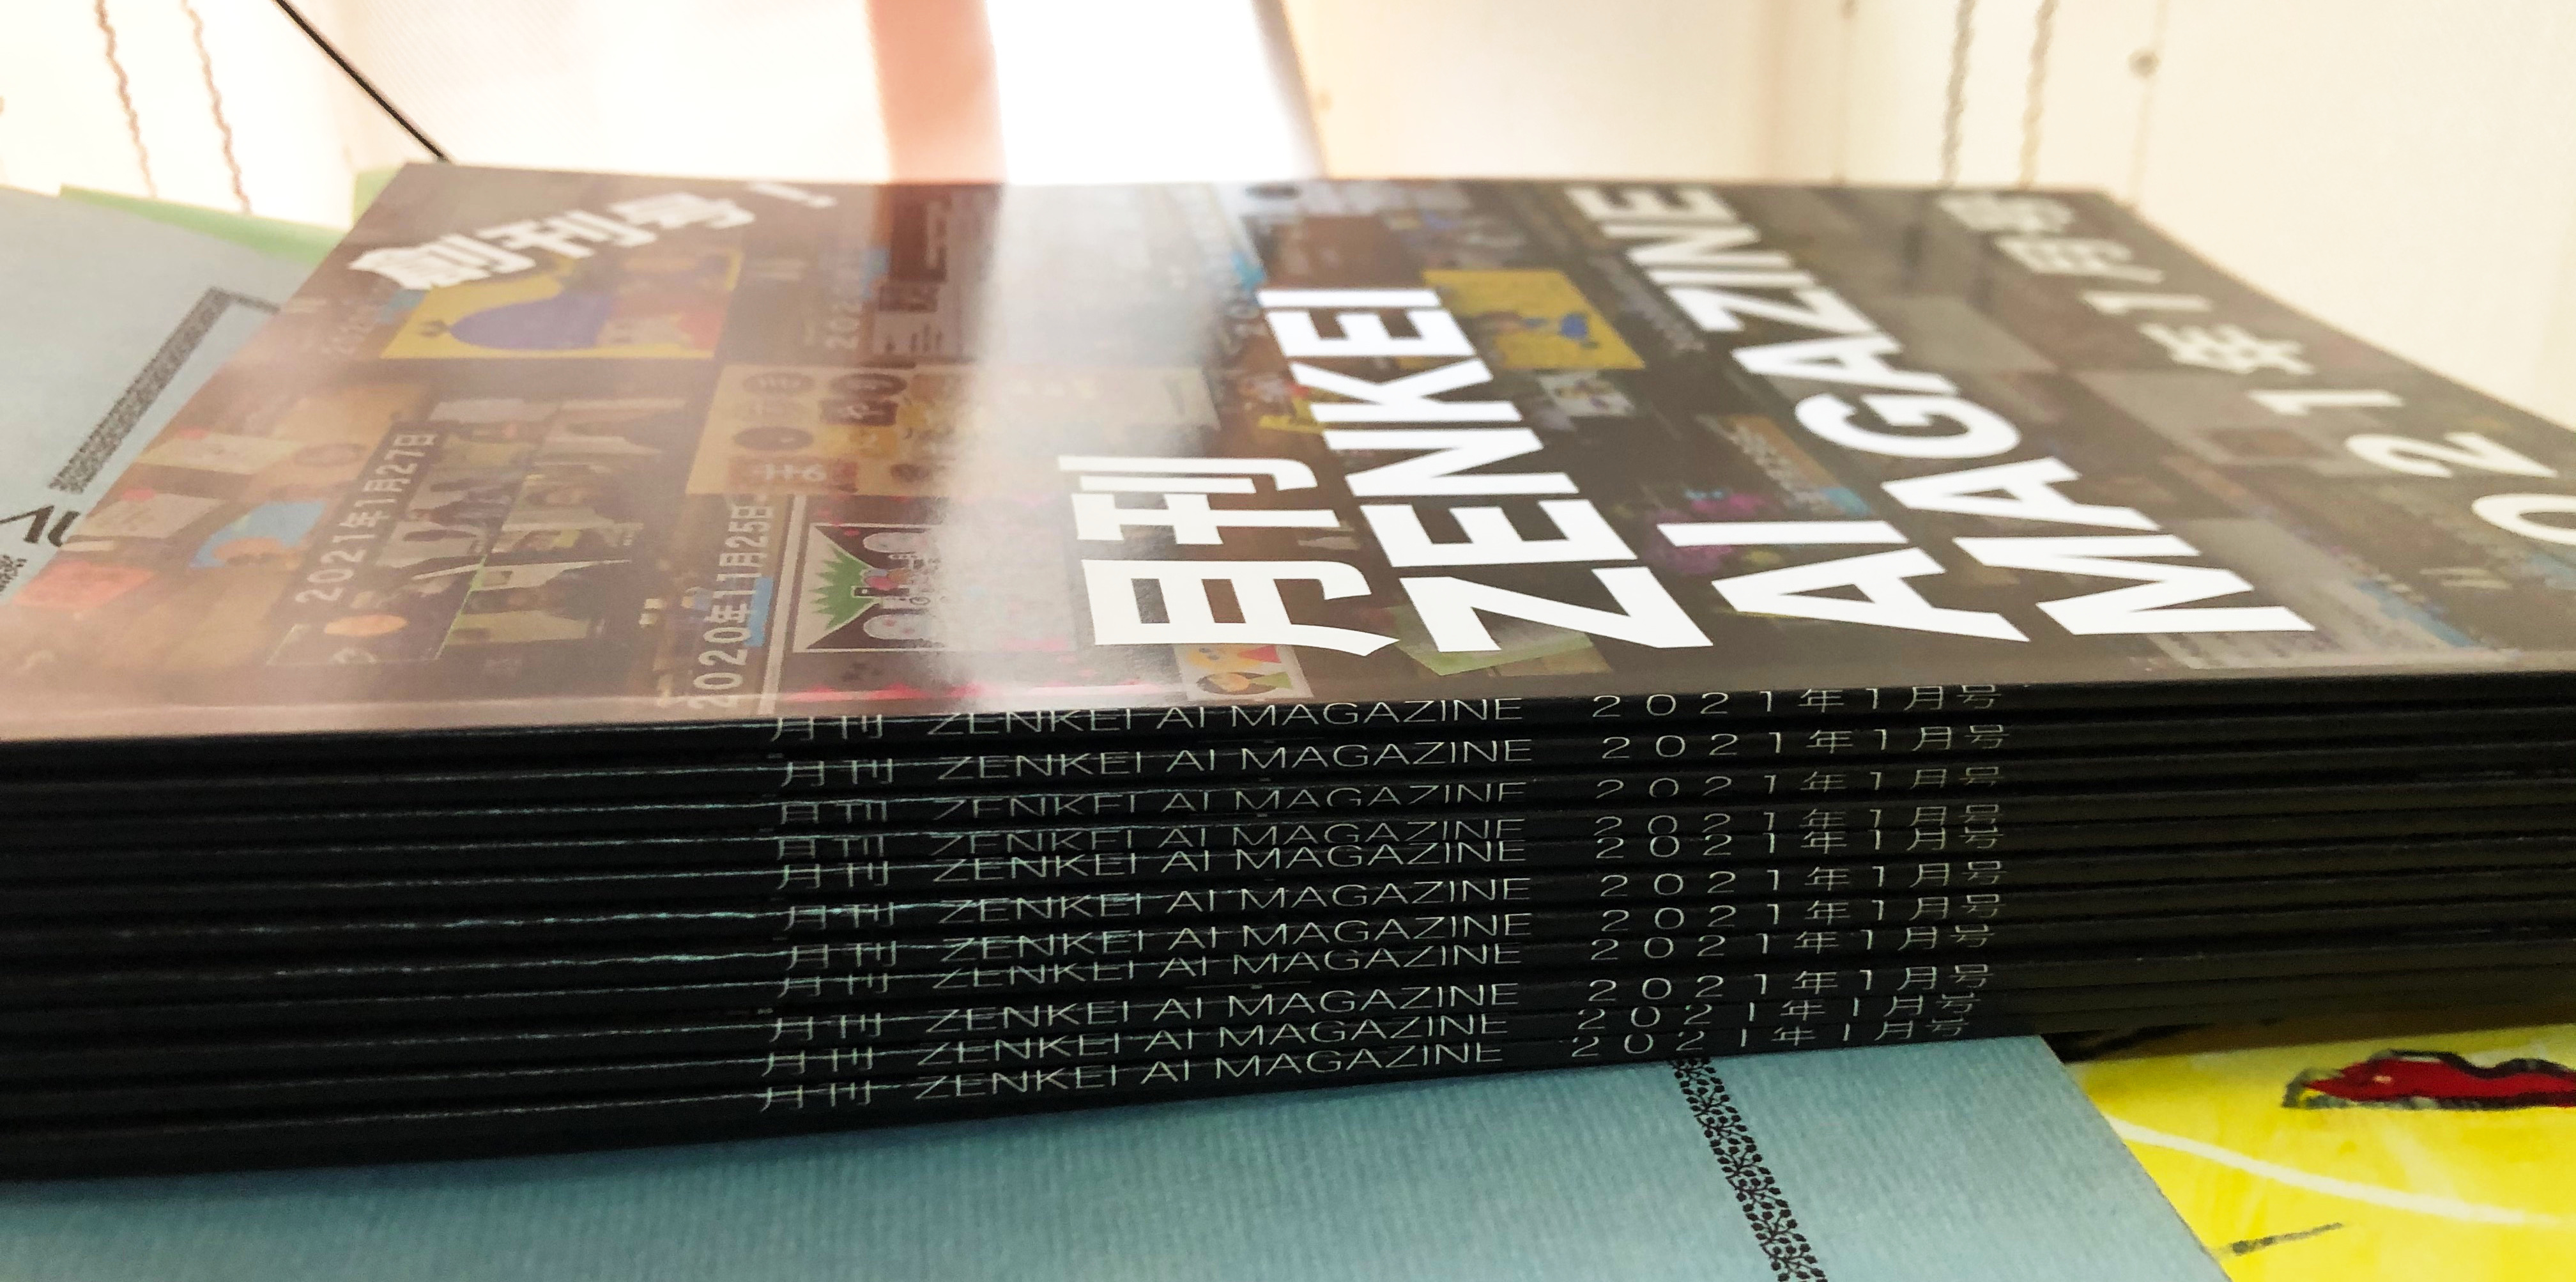
\includegraphics[width=1.5\textwidth,height=0.6\textwidth]
        {images/zam202101-03.jpg}
    };  
  \end{tikzpicture}\\
  \bfseries \Huge \color{white} 第 \thechapter 章 \color{black}\\
} % label
{0pt} % spacing
{} % in front of the title
[]

\chapter{はじめに}
\label{ch:zenza}
\thispagestyle{fancy}

ZENKEI AI FORUM (ZAF) 当日(2021年3月31日)は
メインの「チーム・ホンダ」による発表を控えて、
場をあたためるという本来の意味での「前座」として
『ZAM 創刊号の印刷版がきました!』というはなしをしました。

\begin{multicols}{2}

\section*{ZAM 創刊号、印刷版きました!}
前回2月の ZAF で無事に創刊された ZENKEI AI MAGAZINE
『ZAM 1月号』
(\url{https://zenkei-ai-forum.github.io/ZAM202101/})
ですが、その後自分へのご褒美として10部ほど印刷してみました。
印刷を頼んだのは『ちょ古っ都製本工房』さん
(\url{https://www.chokotto.jp/})
で、内容は以下の通りです。
{\small
\begin{itemize}
  \item B5 30ページ
  \item 本文
  \begin{itemize}
    \item モノクロ印刷(スタンダード)
    \item 上質70kg
  \end{itemize}
  \item 表紙
  \begin{itemize}
    \item 色上質最厚口・135kg(高品質フルカラー印刷)
    \item オプション加工 表2・3 モノクロ印刷
  \end{itemize}
  \item 納期 10営業日コース
  \item 印刷部数 10冊
\end{itemize}
}
税込で 2,230 円でした。

この印刷版 ZAM 創刊号が先日(3月28日)届きました!

 % 全角スペース

\begin{tikzpicture}[remember picture, overlay]
  \node[xshift=4.2cm,yshift=-3.2cm] at (current page.center){
    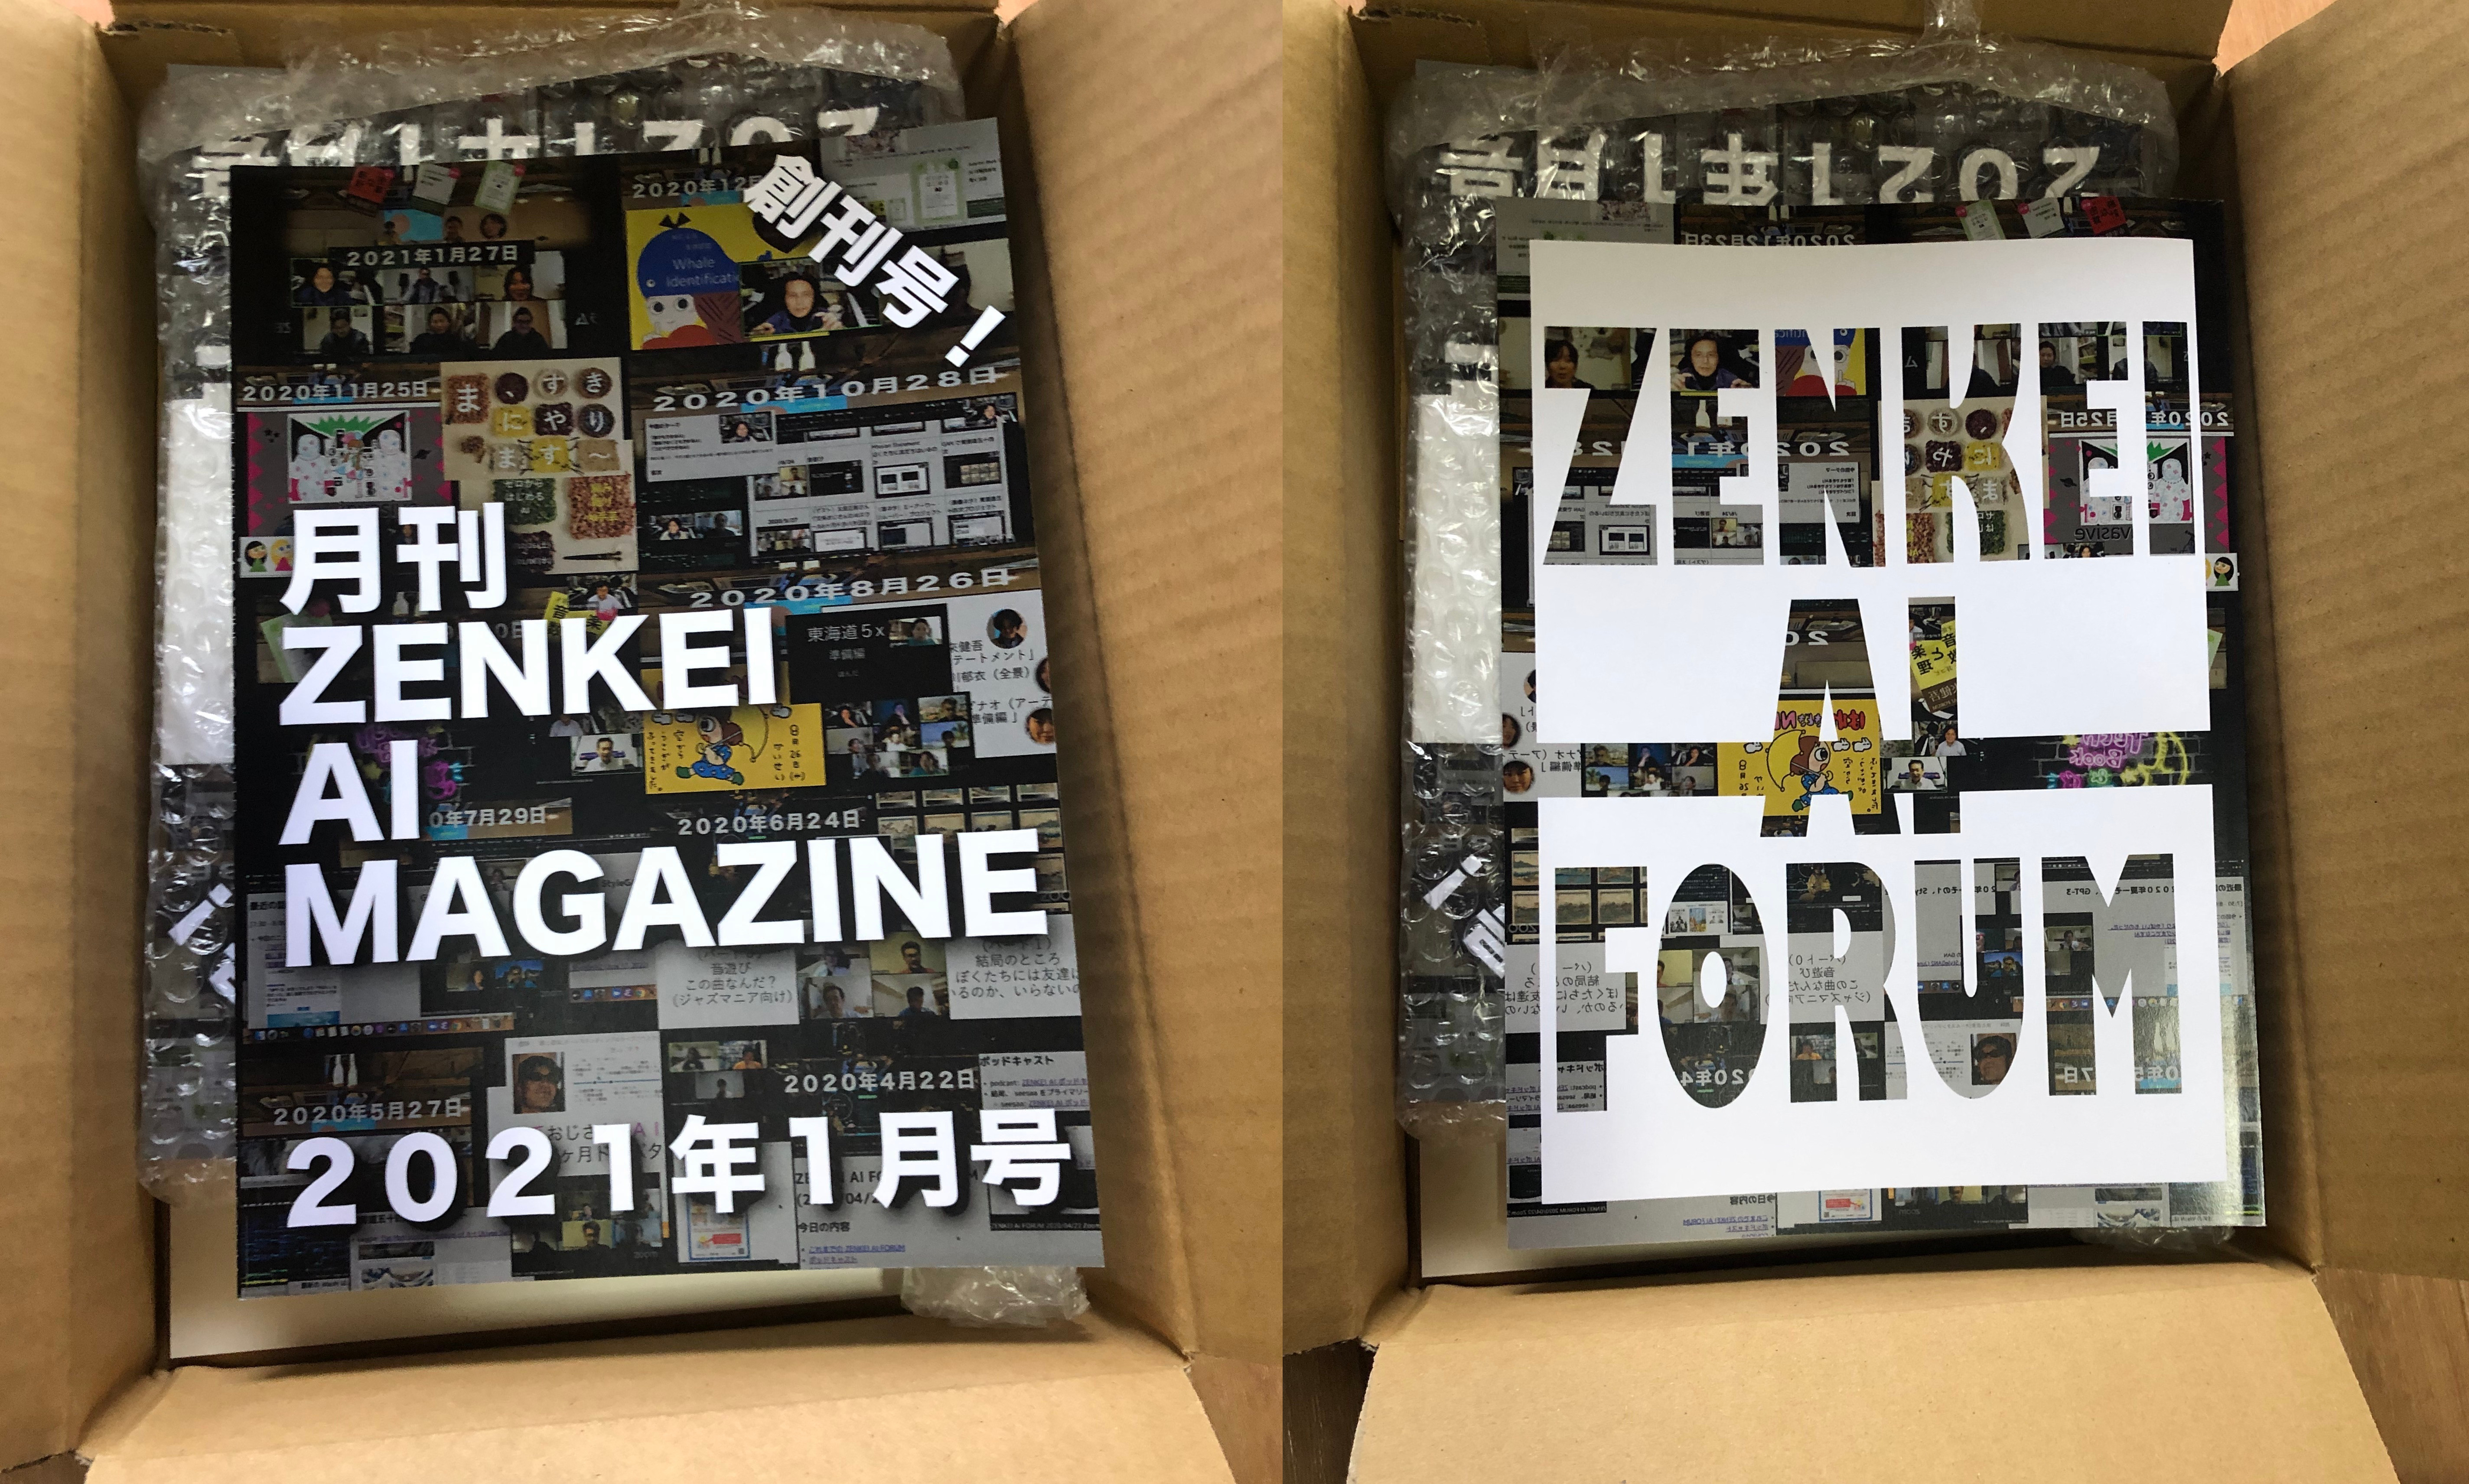
\includegraphics[width=0.54\textwidth]{images/zam202101-01-02.jpg}
  };  
\end{tikzpicture}

\vspace{4.0cm}

\noindent
今回は10冊しか刷りませんでした(余丁1部)。
なので ZAF 1月のイベントの関係者、つまり講演者であり執筆者と、
当日 ZOOM および YouTube での参加者のみなさまにお礼として配ったら
残り2冊しか余りませんでした。
欲しい人、いますか?1冊 1,500 円です!(これで元が取れる!!)
……というのは冗談です。
今後 ZAF の活動に、例えば『数理クイズ』の賞品にしようかな、と思ってます。

\end{multicols}

%\newpage

\titleformat{\chapter}[block]
{\gtfamily \Huge} % style
{
  \begin{tikzpicture}[remember picture, overlay]
    \node[xshift=0cm,yshift=-4.2cm] at (current page.north){%
      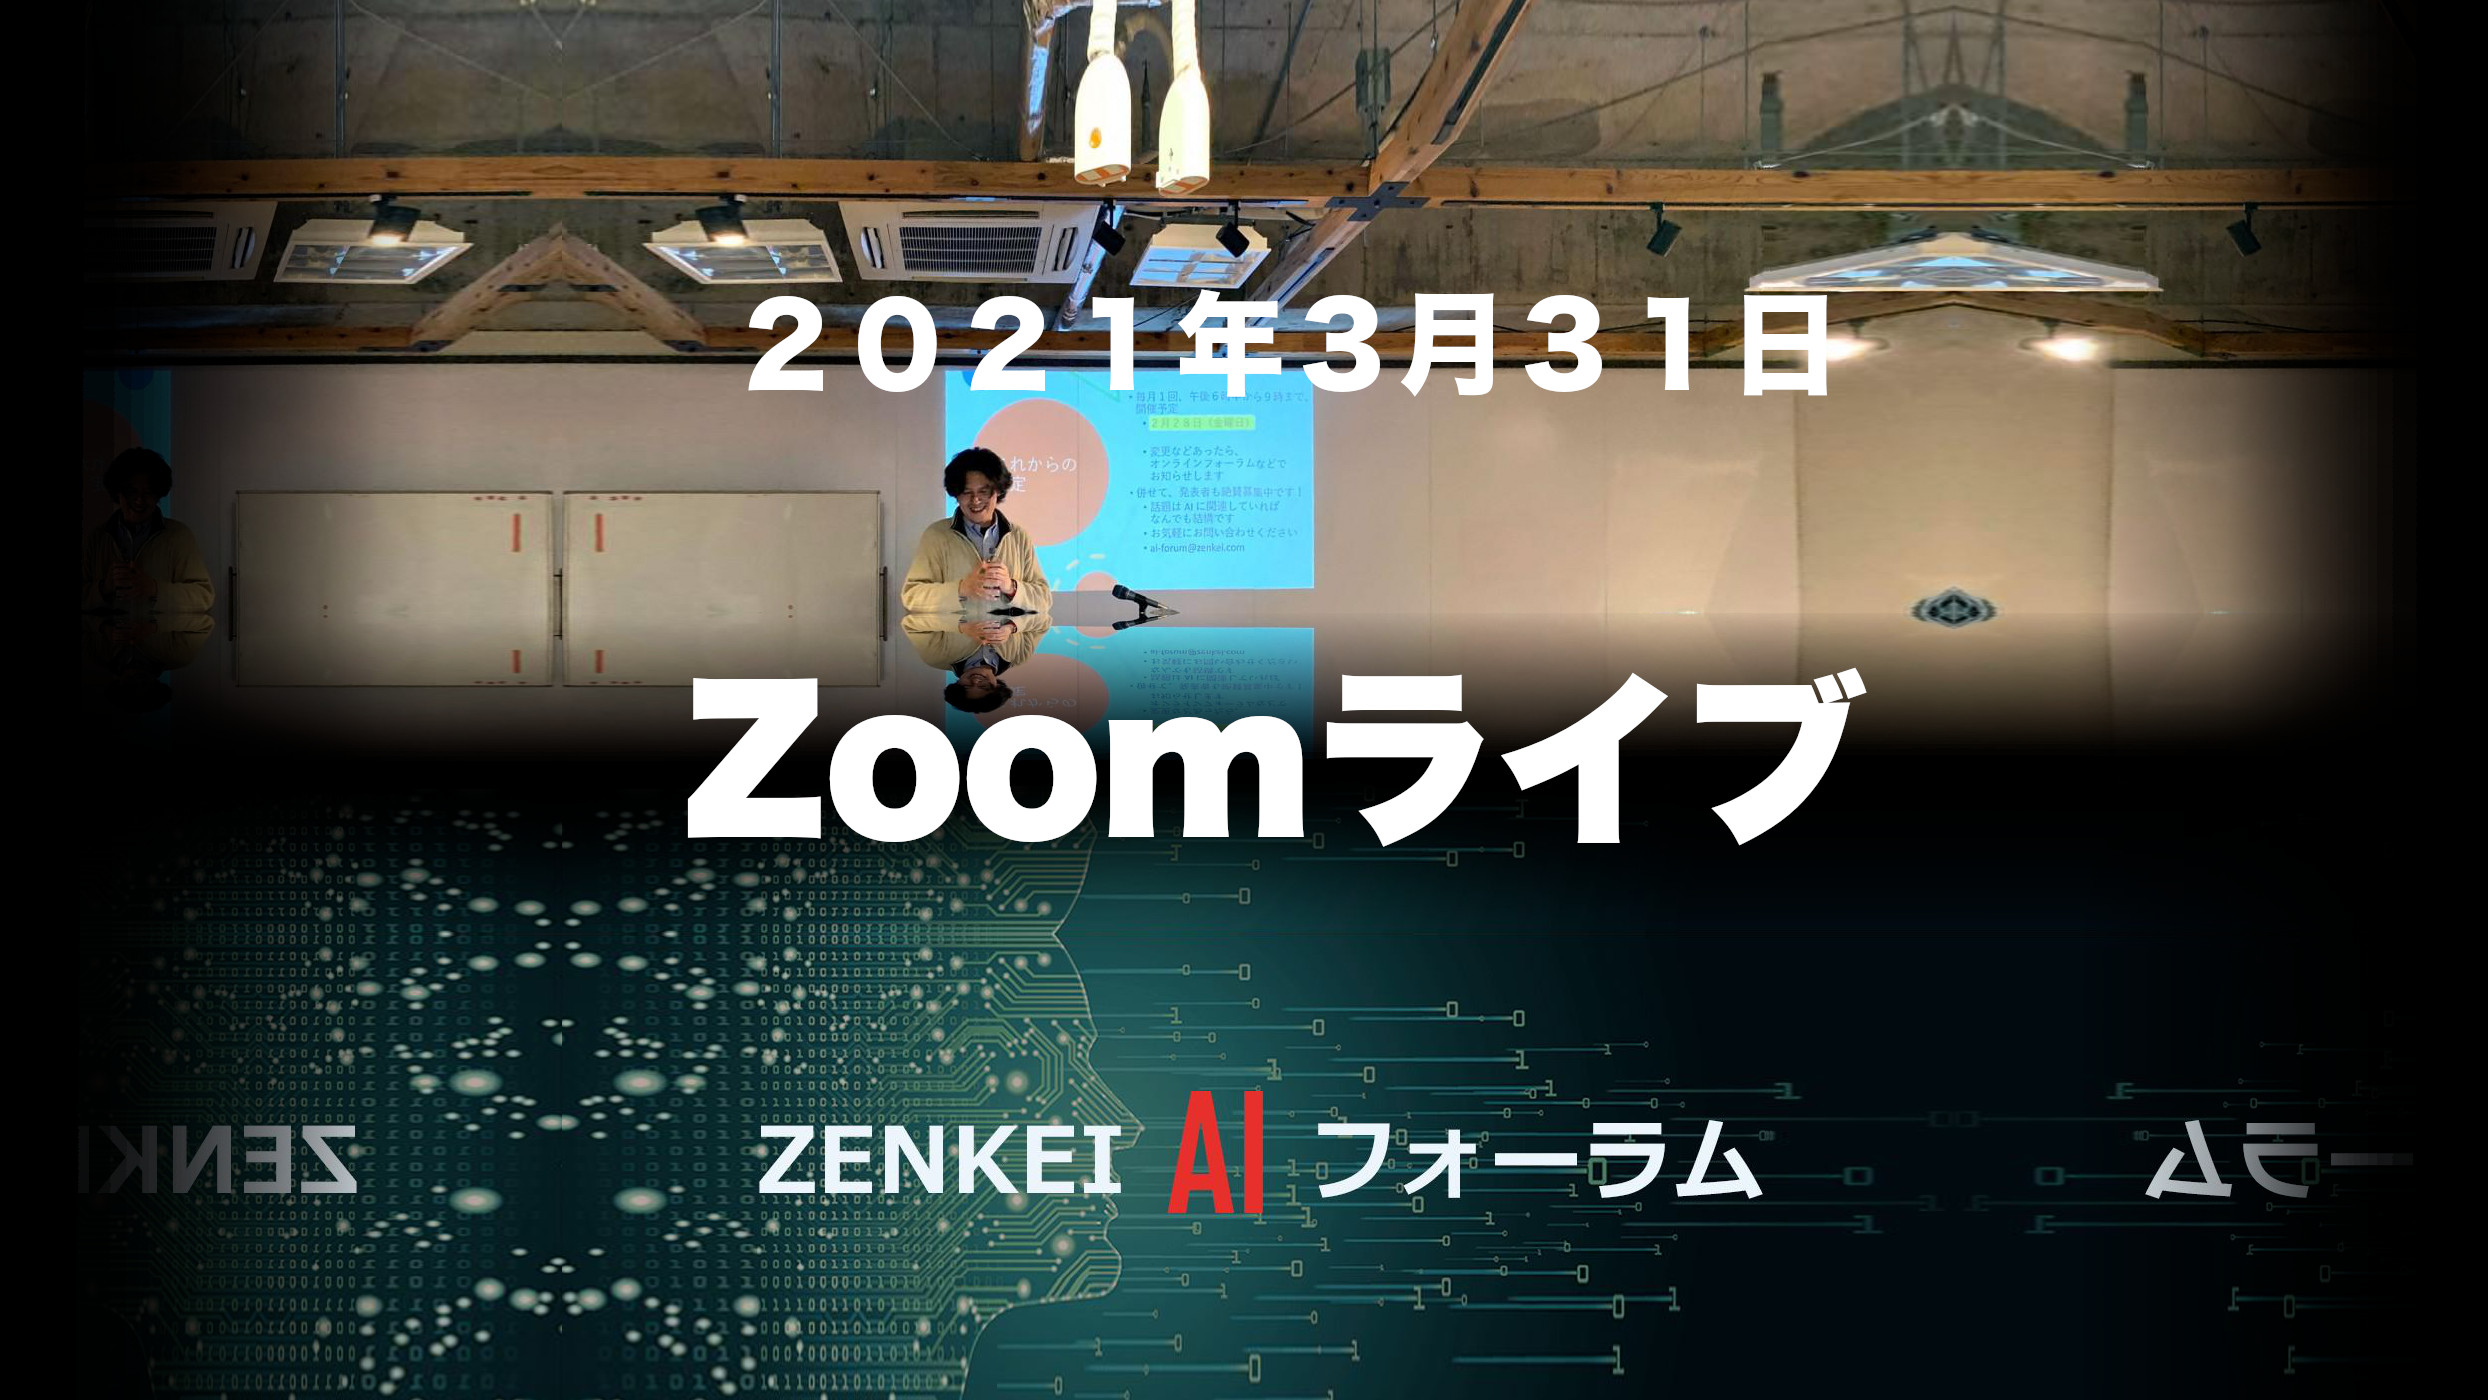
\includegraphics[width=1.5\textwidth,height=0.6\textwidth]
        {images/ZENKEI_AI_FORUM_zoom_20210331-notitle-2488x1400.jpg}
    };  
  \end{tikzpicture}\\
  \bfseries \Huge \color{white} 第 \thechapter 章 \color{black}\\
} % label
{0pt} % spacing
{} % in front of the title
[]

% reset to default (like) format
%\titleformat{\chapter}[block]
%{\gtfamily \Huge} % style
%{\huge 第 \thechapter 章\\} % label
%{0pt} % spacing
%{} % in front of the title
%[]

\chapter[コンピュータ会話教室(市來健吾)]{コンピュータ会話教室(市來健吾)\\第1回: for ループ}
\label{ch:ichiki}
\thispagestyle{fancy}

コンピュータが人間の能力を(画像認識など一部のタスクで)凌駕しつつある2021年の今こそ、
みなさんコンピュータと会話してみませんか?コンピュータ会話教室の開幕です!


\begin{multicols}{2}

\section*{はじめに}
「語学学習」は生涯学習の文脈で多くの人々の関心にあります。
街の本屋さんには語学コーナーが大きな場所を取ってますし、
アマゾンで検索すると膨大な数の本が出てきます。

普通「語学」というと「英会話」ですね。
英語ができればとりあえず世界を歩くことはできそうです。
将来を見て、また、日本という立地を考えて、
やはり今は「中国語」という方もいらっしゃるでしょう。

ここに別の視点、 ZENKEI AI FORUM 的視点として、
近い将来、人間よりも高い能力を獲得するであろう、
地球上の種族「コンピュータ」と会話できるって、素敵じゃないですか?

(と、ちょっとキャッチーなコピーを書いてみました。
ちなみに『数理クイズ』を企画したのも背景としては同じ気持ちでした。)

\section*{第1回: for ループ}
新企画『コンピュータ会話教室』第1回のお題は『for ループ』です。
「なんで?」と思った人が大半かなと思います。
英語なら "Hello! How are you doing?" とか "This is a pen" なのに、
どうしてコンピュータ会話は『for ループ』から始まるのか、
ちょっと説明しますね。

\section*{コンピュータって何?}
コンピュータ、英語の computer は日本語だと「電子計算機」ですね
(今は誰もこんな風に呼びませんが)。
「電卓」ってありますよね。電卓も計算できます。
では、電卓とコンピュータの違いは何でしょう?
電卓は計算ができますが、逆にいうと、計算しかできません。
もっというと、1度に1つの計算しかできません。
一方コンピュータは「プログラム」ができます。

\section*{プログラムとは}
さて、それでは「プログラム」って何でしょうか?
結論から言うと、これがコンピュータと人間がコミュニケーションするための「言語」です。
ということで『コンピュータ会話教室』はプログラム言語を喋れるようになることが目的の
会話教室ということになります。
『英会話教室』が英語が喋れるようになることが目的のように。
少しは親しみを感じてもらえたでしょうか。

とはいえ、プログラムは人と人のコミュニケーションの言語ではなく、
人とコンピュータのコミュニケーションのための言語で、
人の方が少しコンピュータに寄り添ったものです。
つまり基本的にはプログラムは、
コンピュータに対する指示文書です。

電卓は、1つの指示をその場で受け取って(ボタンを叩いて)、
その場で答えます(7セグの LED で結果を表示して)。
コンピュータは、指示の書かれた文書(プログラム)を受け取って、
その指示に沿って計算し、その答えを返します。

\begin{tikzpicture}[remember picture, overlay]
  \node[xshift=-4.2cm,yshift=-6.3cm] at (current page.center){
    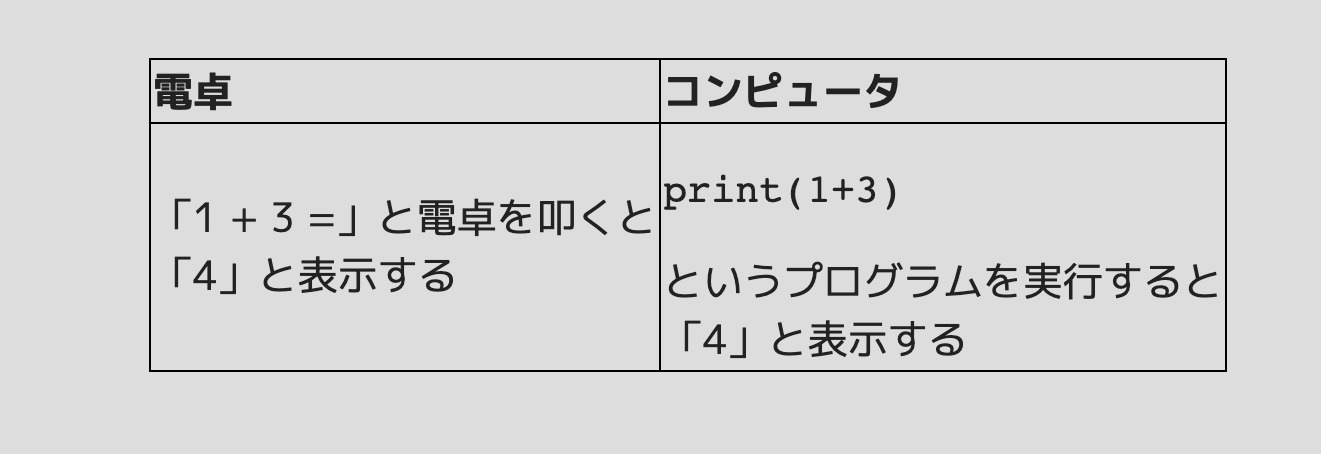
\includegraphics[width=0.54\textwidth]{images/table-01.jpg}
  };  
\end{tikzpicture}

\vspace{1.5cm}

\section*{プログラムのパワー}
これだけ見るとプログラムの凄さが分かりませんね。
しかしプログラムには沢山の指示を書き込むことができて、
それを受け取ったコンピュータはその指示を全ていっぺんに計算することができます。
「仕事の効率化」というやつですね!

\begin{tikzpicture}[remember picture, overlay]
  \node[xshift=4.2cm,yshift=7.0cm] at (current page.center){
    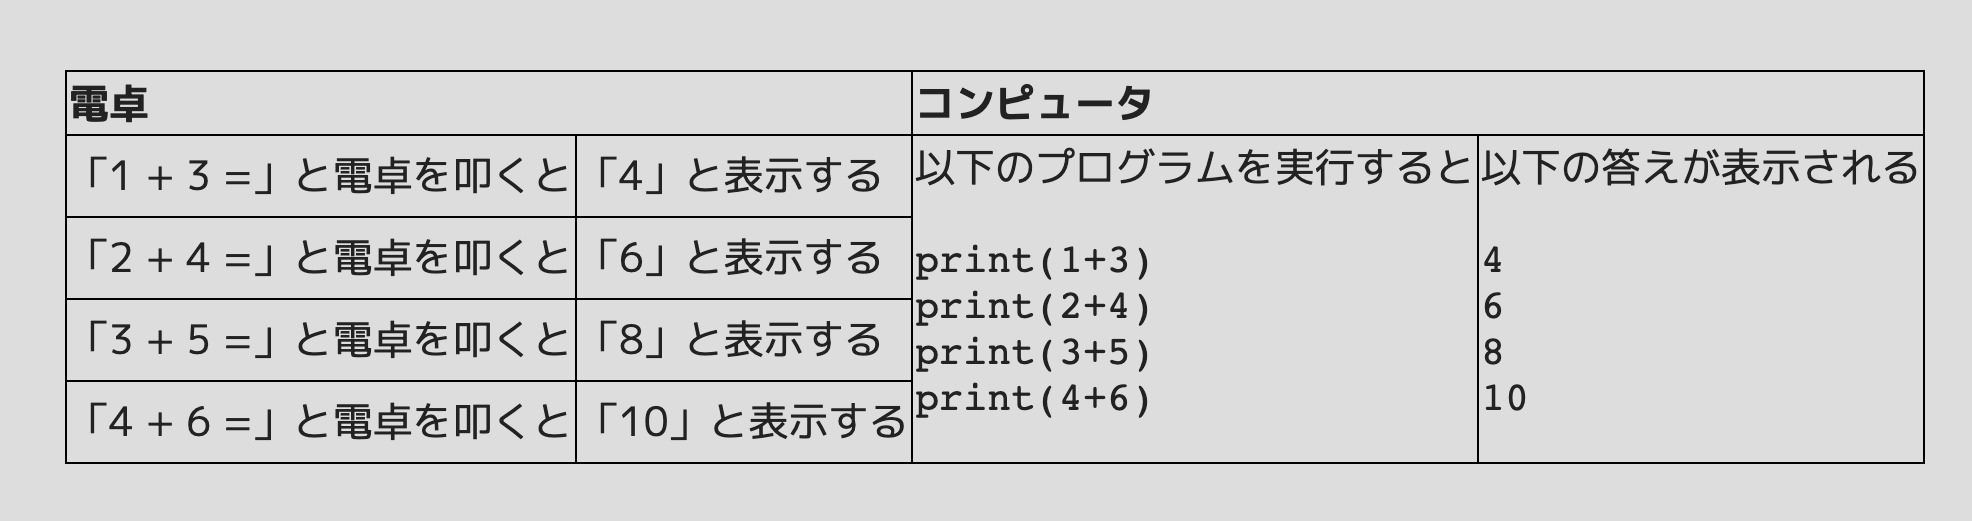
\includegraphics[width=0.54\textwidth]{images/table-02.jpg}
  };  
\end{tikzpicture}

\vspace{1.5cm}

\noindent
すごい、すごい、めでたし、めでたし。
しかし私たちが、いつもいつも「1+3」とか「4+6」が計算したいわけではありません。
しかしプログラムは、そこに書かれた指示を一般化できます。
つまりプログラムには「変数」を使うことができます。

\begin{tikzpicture}[remember picture, overlay]
  \node[xshift=4.2cm,yshift=1.6cm] at (current page.center){
    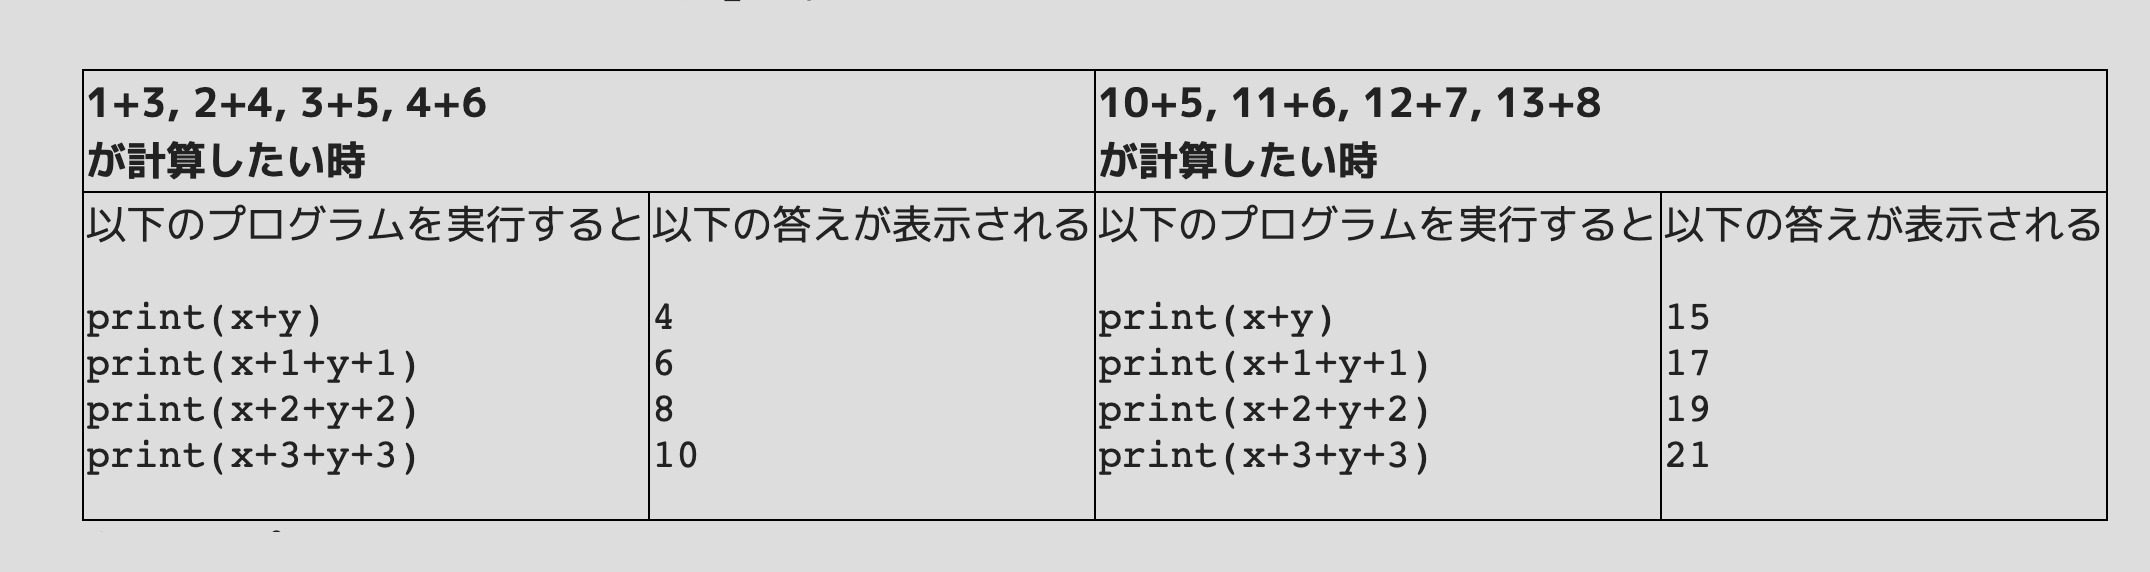
\includegraphics[width=0.54\textwidth]{images/table-03.jpg}
  };  
\end{tikzpicture}

\vspace{1.5cm}

\noindent
ここで注目するポイントは、プログラムは全く同じということです。
いちいちプログラムを書き換えることなく、いろんな足し算が計算できます!
すごい、すごい、めでたし、めでたし。

しかし4行も「print」とか打ち込みたくないですよね。
人は強欲なもので、便利になってもすぐに慣れてしまいます。
しかしこのことは(今の文脈においては)全然悪いことではありません。
効率化は正義、不精はプログラマーの美徳です。


\section*{for ループ}
お待たせしました。ここで出てくるのが『for ループ』です。
個人的には「プログラムの本質は『for ループ』だ!」というくらいに思ってます。
(もう1つのプログラムの本質はサブルーチン、あるいは関数ですね。)
『for ループ』とは、繰り返し処理を簡単に書く構文、イディオムですね。
(語学っぽい!)

\begin{tikzpicture}[remember picture, overlay]
  \node[xshift=-4.2cm,yshift=8.0cm] at (current page.center){
    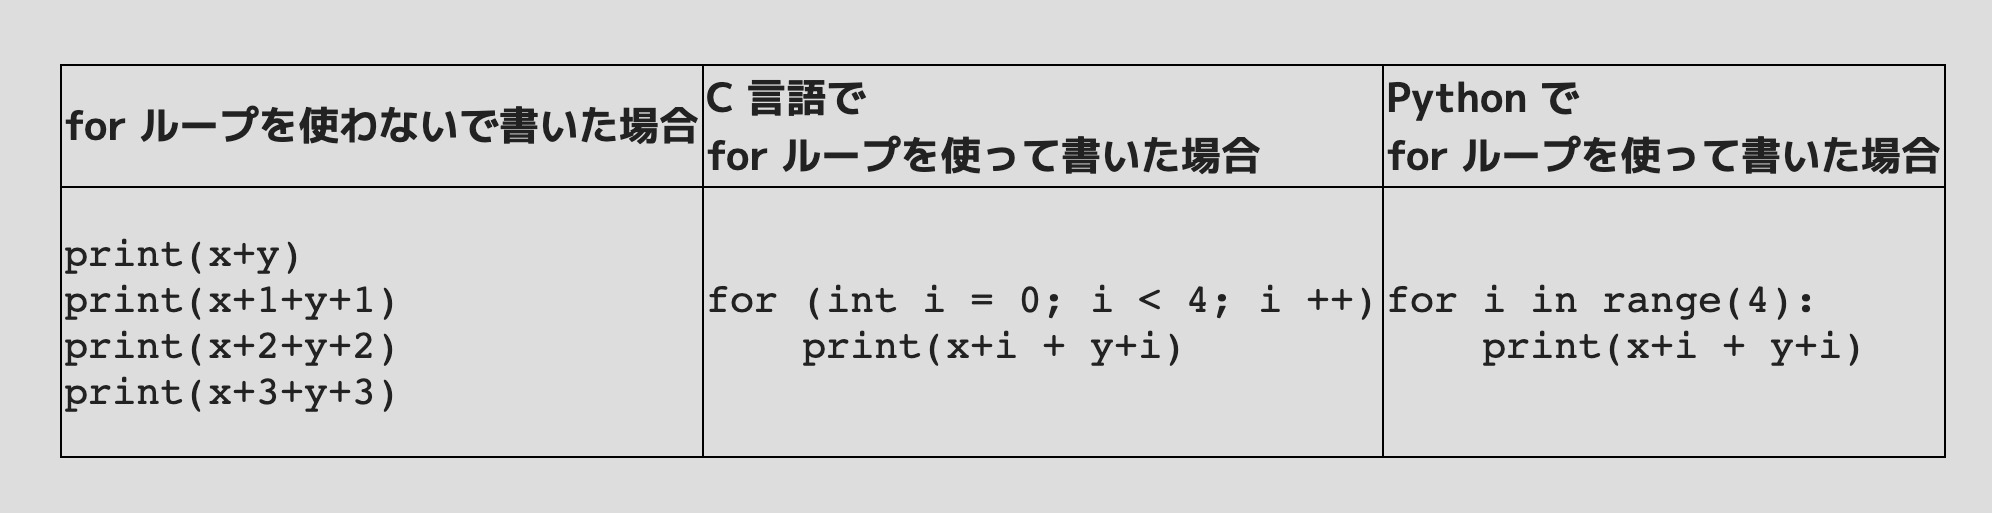
\includegraphics[width=0.54\textwidth]{images/table-04.jpg}
  };  
\end{tikzpicture}

\vspace{1.5cm}

\section*{C言語編}
C 言語の for ループは(条件など具体的に書かれているので)分かりやすいですね。
\begin{lstlisting}
for (int i = 0; i < 4; i ++) {
    // 繰り返し処理
}
\end{lstlisting}
\noindent
ここで {\ttfamily for} につづくカッコの中の、
セミコロン(;)で区切られた3つの部分の意味を説明します。
最初の {\ttfamily int i = 0} は
「繰り返し処理」に入る前に1度だけ呼ばれる処理です。
今の場合、変数 {\ttfamily i} を準備して、
値 {\ttfamily 0} を代入しています。
2つ目の部分 {\ttfamily i < 4} は「繰り返し処理」が継続する条件です。
つまり変数 {\ttfamily i} の値が {\ttfamily 4} よりも小さい限り
処理が繰り返されることになります。
最後の部分 {\ttfamily i ++} は各「繰り返し処理」が終わった後に実行される処理です。
今の場合「繰り返し処理」が終わった後に、その都度変数{\ttfamily i}
の値を {\ttfamily 1} ずつ増やしていきます。


具体的な処理の流れを見ていきましょう。
「繰り返し処理」が変数 {\ttfamily i} の値を表示する処理、
つまり {\ttfamily printf(i)} を実行する場合を考えます。
\begin{lstlisting}
for (int i = 0; i < 4; i ++) {
    printf(i);
}
\end{lstlisting}
{\small
  \begin{itemize}
  \item まず変数 {\ttfamily i} に {\ttfamily 0} が代入される
  \item 繰り返し処理が実行され  {\ttfamily 0} と表示される
  \item {\ttfamily i ++} が実行され {\ttfamily i} が1つ増え
    {\ttfamily 1} となる
  \item {\ttfamily i} は条件を満たすので、繰り返し処理は継続する
    (今 {\ttfamily i} は {\ttfamily 1} が入っている)
  \item 繰り返し処理が実行され {\ttfamily 1} と表示される
  \item {\ttfamily i ++} が実行され {\ttfamily i} が1つ増え
    {\ttfamily 2} となる
  \item {\ttfamily i} は条件を満たすので、繰り返し処理は継続する
    (今 {\ttfamily i} は {\ttfamily 2} が入っている)
  \item 繰り返し処理が実行され {\ttfamily 2} と表示される
  \item {\ttfamily i ++} が実行され {\ttfamily i} が1つ増え
    {\ttfamily 3} となる
  \item {\ttfamily i} は条件を満たすので、繰り返し処理は継続する
    (今 {\ttfamily i} は {\ttfamily 3} が入っている)
  \item 繰り返し処理が実行され {\ttfamily 3} と表示される
  \item {\ttfamily i ++} が実行され {\ttfamily i} が1つ増え
    {\ttfamily 4} となる
  \item {\ttfamily i} は条件を満たさないので、繰り返し終了
  \end{itemize}
}
以上がこの for ループの具体的な処理の流れです。

\section*{Python編}
ZAF の公式プログラム言語 Python で
先の C 言語の for ループを書き換えると以下のようになります。
\begin{lstlisting}
for i in range(4):
    print(i)
\end{lstlisting}

\noindent
慣れるまでは、これをイディオムとして丸暗記してもいいですが(語学教室っぽいですね!)
ここでは簡単にその中身を説明しましょう。

{\ttfamily range(4)} はイテレータ (iterator) と呼ばれるものです。
このイテレータは for ループを抽象的に扱えるようにするためのオブジェクトで、
「順番に値を出してくれるオブジェクト」くらいのイメージです。
具体的には配列 (Array) をそのまま思い浮かべてもいいでしょう
(実際、イテレータが導入される前の Python では {\ttfamily range(4)} は
{\ttfamily [0, 1, 2, 3]} と言う配列でした。)
この Python の for ループの構文
\begin{lstlisting}
for (変数) in (イテレータ):
    # 繰り返し処理
\end{lstlisting}
の具体的な処理の流れは、
{\small
  \begin{itemize}
  \item 「イテレータ」から順番に要素を取り出して
  \item 「変数」に代入して
  \item 「繰り返し処理」を行います。
  \end{itemize}
}

この Python で出てきたイテレータは結構奥が深くて、興味深いです。
わたしは元々 C 言語でプログラムを学んできて、
長い間この素朴で原始的な C の for ループで十分だと思ってきました。
しかし Python を本格的に使い始めて、
いろいろ使っていくうちに、少し考え方を改めて、
イテレータによって for ループが一段階、抽象化(一般化)されたと感じています。
この\ruby{辺}{あた}りの感覚を知りたい方は、是非、
Python のエキスパートである Ned Batchelder さんのすごく印象的な
30分の講演ビデオをご覧になってください。
きっと眼から鱗が落ちる体験をすると思います。
\url{https://youtu.be/EnSu9hHGq5o}

\begin{tikzpicture}[remember picture, overlay]
  \node[xshift=-4.2cm,yshift=-1.3cm] at (current page.center){
    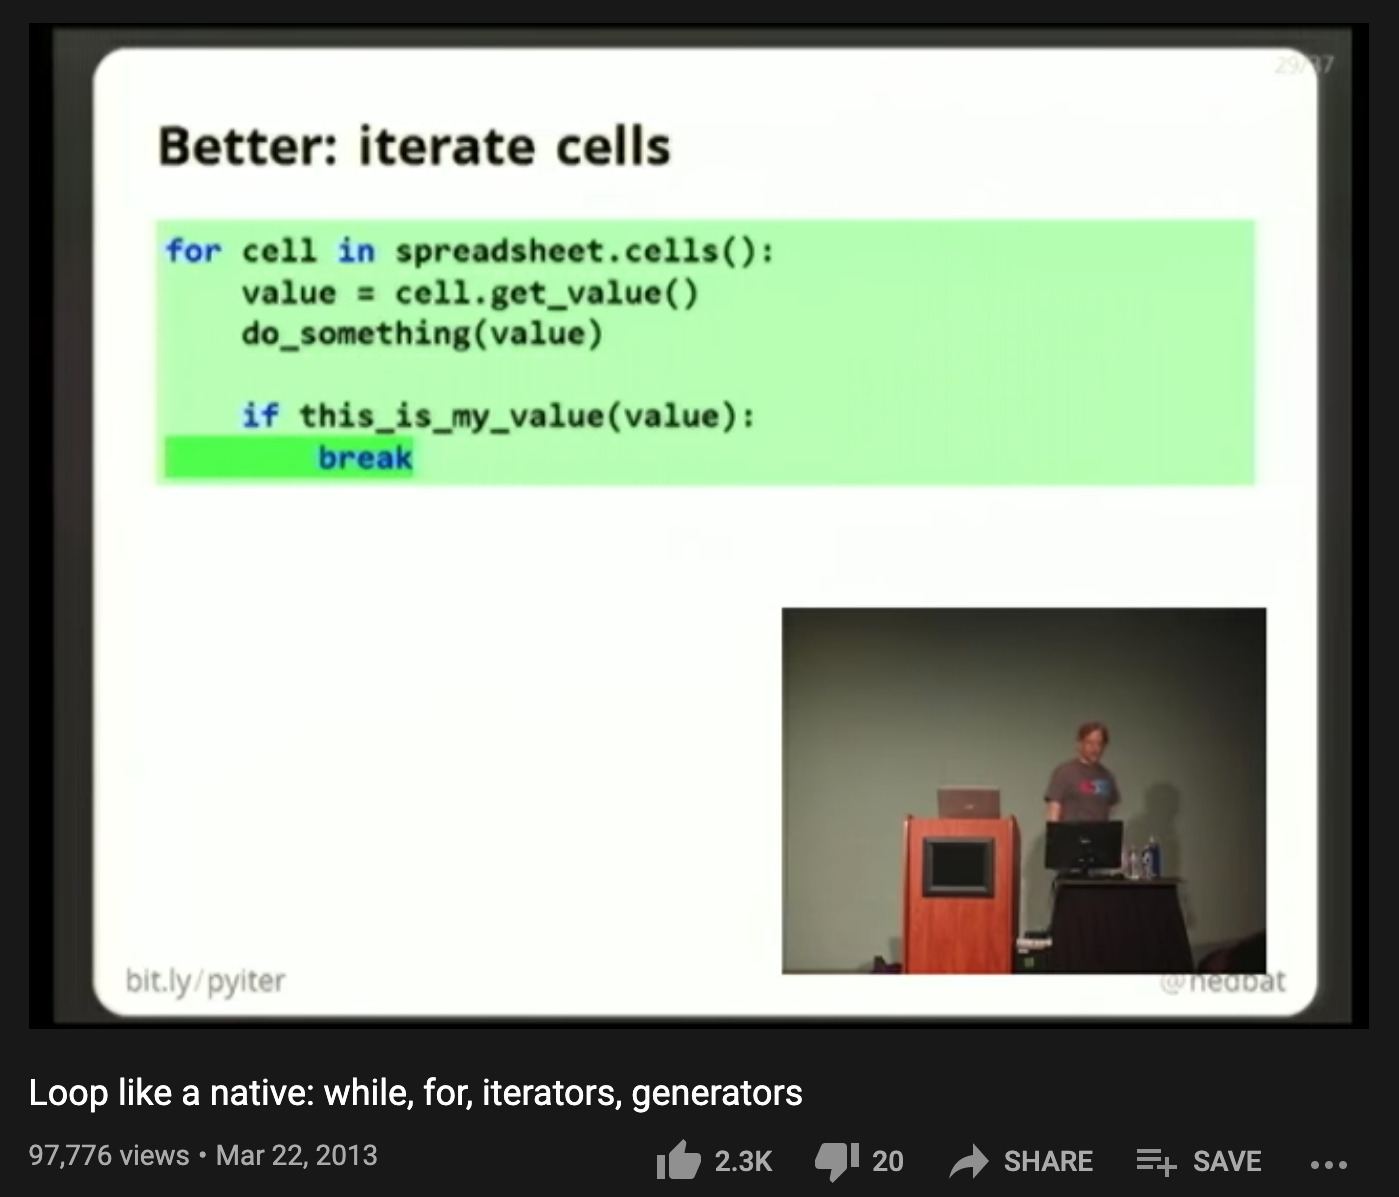
\includegraphics[width=0.5\textwidth]{images/youtube-ned.jpg}
  };  
\end{tikzpicture}

\vspace{5.5cm}


\section*{ベクトル}
実は今日あえて『for ループ』を取り上げたのは
(温めていた『コンピュータ会話教室』という企画の他に)
もう1つの理由があります!

みなさん配列 (Array) はご存知ですよね?
上で少し言及しましたが、たくさんの数字を格納する入れ物みたいなものです。
ところでベクトル (vector) は知ってますか?
高校の数学の授業を思い出せば「あの矢印ね」となります(よね)。
2次元空間(平面)のベクトル $\bm{v}$ は2つの成分 $(x, y)$ で表される矢印に対応し、
3次元空間のベクトル $\bm{w}$ は 3つの成分 $(x, y, z)$ で表される矢印に対応します。
今は数学の授業ではなく『コンピュータ会話教室』なので、
それぞれ長さが2とか3の配列という認識で十分です。

\section*{行列}
では次に行列 (matrix) はご存知ですか?
高校でベクトルと一緒に習ったはずです。
「1次変換」とか「ベクトルの回転」とか覚えてますか?
2次元空間(平面)の行列 $\mathsf{A}$ は $2\times 2$ 個の要素(数字)を持つ量です。
その4つの成分は $(A_{xx}, A_{xy}, A_{yx}, A_{yy})$ です。
原点を中心に角度 $\theta$ の回転を表す行列は以下のように書けます。
\begin{equation*}
  \mathsf{A}
  =
  \left[
  \begin{array}{cc}
    A_{xx} & A_{xy} \\
    A_{yx} & A_{yy}
  \end{array}
  \right]
  =	
  \left[
  \begin{array}{cc}
    \cos\theta & -\sin\theta \\
    \sin\theta & \cos\theta
  \end{array}
  \right]
\end{equation*}
この辺で頭痛がしてきた人がいるかもしれませんね。
「あれ、マイナスは右上の $\sin$ だったっけ?」とか、記憶が怪しくなってきます。
数学は丸暗記するものではなく、考えると分かるものなので、
$\sin$ と $\cos$ の並びや、その符号に自信が持てなくなっても心配は要りません!

この行列が本当に回転行列なのかを確認するために、
行列 $\mathsf{A}$ とベクトル $\bm{x}$ の積の定義を確認しておきましょう。
\begin{equation*}
  \mathsf{A}\cdot\bm{x}
  =
  \left[
  \begin{array}{cc}
    A_{xx} & A_{xy} \\
    A_{yx} & A_{yy}
  \end{array}
  \right]
  \cdot
  \left[
  \begin{array}{c}
    x \\
    y
  \end{array}
  \right]
  =	
  \left[
  \begin{array}{c}
    A_{xx} x + A_{xy} y \\
    A_{yx} x + A_{yy} y
    \end{array}
  \right]
\end{equation*}
この式に先の回転行列と、
ベクトルの成分 $\bm{x} = (x, y)$ を代入すると、以下のようになりますね。
\begin{equation*}
  \mathsf{A}\cdot\bm{x}
  =	
  \left[
  \begin{array}{c}
    \cos\theta\ x - \sin\theta\ y \\
    \sin\theta\ x + \cos\theta\ y
  \end{array}
  \right]
\end{equation*}
ここで $\bm{x}$ に簡単な場合を考えて、つまり
$\bm{x} = (1, 0)$ の時(右向きベクトル)の場合と
$\bm{x} = (0, 1)$ の時(上向きベクトル)の場合
の具体的な結果をみてみよう。
上の結果から
$\bm{x} = (1, 0)$ の時は $(\cos\theta, \sin\theta)$ というベクトル、
$\bm{x} = (0, 1)$ の時は $(-\sin\theta, \cos\theta)$ というベクトル
がそれぞれ得られます。
つまり、それぞれ実際に $\theta$ 回転していることが確認できました!

\begin{tikzpicture}[remember picture, overlay]
  \node[xshift=-4.2cm,yshift=3.1cm] at (current page.center){
    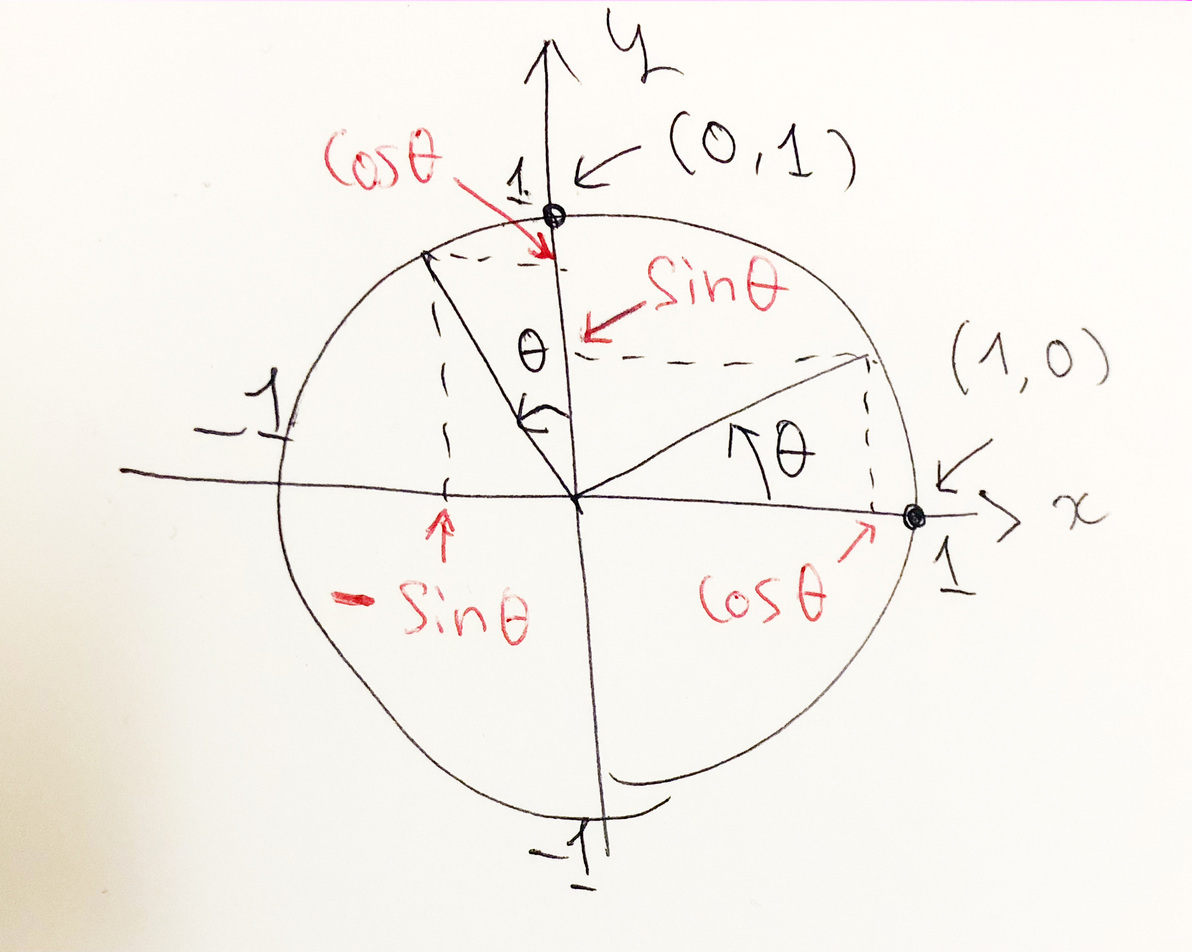
\includegraphics[width=0.5\textwidth]{images/fig-rotation-2d.jpg}
  };  
\end{tikzpicture}

\vspace{4.4cm}

\section*{プログラム}
ではここでこの行列とベクトルの積をプログラムにしてみましょう。
ベクトル {\ttfamily vec} を配列で、行列 {\ttfamily A} を2次元配列で書いて
\begin{lstlisting}
vec = [x, y]
A = [[Axx, Axy], [Ayx, Ayy]]
\end{lstlisting}
行列とベクトルの積をプログラムで書くと
\begin{lstlisting}
def mat_vec_prod(A, vec):
  y = [0, 0]
  for i in range(2):
    for j in range(2):
      y[i] += A[i][j] * vec[j]
  return y
\end{lstlisting}
となります。
上で書いた式と比べて確認してみてくださいね。

\section*{行列と行列の積のプログラム}
次に行列と行列の積を考えてみましょう。
これは今みた行列とベクトルの積のシンプルな拡張です。
2つの $2\times 2$ 行列 {\ttfamily A} と {\ttfamily B} の行列積の計算は
\begin{lstlisting}
def mat_mat_prod(A, B):
  C = [[0, 0], [0, 0]]
  for i in range(2):
    for j in range(2):
      for k in range(2):
        C[i][j] += A[i][k] * B[k][j]
  return C
\end{lstlisting}
となります。
(ここでは、こういうものだと思ってください。)
上のプログラムに出てくる {\ttfamily range(2)} の {\ttfamily 2} は
今考えている空間が2次元だからです。
任意の次元 {\ttfamily n} に対する行列積は
\begin{lstlisting}
def mat_mat_prod(A, B):
  C = [[0]*n for _ in range(2)]
  for i in range(n):
    for j in range(n):
      for k in range(n):
        C[i][j] += A[i][k] * B[k][j]
  return C
\end{lstlisting}
となります。
({\ttfamily n} 次元行列 {\ttfamily C} の初期化はこう言うものだと思ってください。)
ちなみに、そこで出てくる {\ttfamily range(2)} は
{\ttfamily C} が行列だから、つまりインデックスが2つだからです。


\section*{突然の『数理クイズ』}
さて、ここからが本題(えっ?)
今月の数理クイズです!
{\ttfamily n} が大きい時、
行列と行列の積の計算に必要な計算量はどうなるでしょう?
上に書いた通り、素朴に実装すると計算量は $O(n^3)$ となります。
クイズは
\begin{quote}
  \textgt{\bfseries \sffamily \large
    $n$ が大きい時 $O(n^3)$ より効率的に行列積を計算できるでしょうか?
    }
\end{quote}
です。
みなさんの回答、お待ちしてます!

\end{multicols}


\newpage

\titleformat{\chapter}[block]
{} % style
{} % label
{0pt} % spacing
{} % in front of the title
[]
\chapter[東海道5X(ホンダナオ)]{}
\label{ch:honda}

\pagestyle{fancy}
\fancyhf{} % 既定設定をリセット
\renewcommand{\headrulewidth}{0pt} % 罫線無し
\fancyfoot[RE]{第4章 東海道5x}
\fancyfoot[LO]{ホンダナオ}
\fancyfoot[LE,RO]{\thepage}

\thispagestyle{fancy}

\AddToShipoutPictureBG*{%
  \AtPageLowerLeft{%
    \includegraphics[width=\paperwidth,height=\paperheight,page=1]%
      {tokaido5x_honda_02_no-page-num.pdf}
  }%
}%

\includepdf[pages=2-10, pagecommand={}]%
  {tokaido5x_honda_02_no-page-num.pdf}

\titleformat{\chapter}[block]
{} % style
{} % label
{0pt} % spacing
{} % in front of the title
[]
\chapter[東海道五⼗ X プロジェクト(大島圭祐)]{}
\label{ch:ooshima}

\pagestyle{fancy}
\fancyhf{} % 既定設定をリセット
\renewcommand{\headrulewidth}{0pt} % 罫線無し
\fancyfoot[RE]{第5章 東海道五⼗ X プロジェクト}
\fancyfoot[LO]{大島圭祐}
\fancyfoot[LE,RO]{\thepage}

\thispagestyle{fancy}

\AddToShipoutPictureBG*{%
  \AtPageLowerLeft{%
    \includegraphics[width=\paperwidth,height=\paperheight,page=1]%
      {ooshima_ed.pdf}
  }%
}%

\includepdf[pages=2-, pagecommand={}]
     %{ooshima.pdf}
     {ooshima_ed.pdf}

\newpage

\AddToShipoutPictureBG*{%
  \AtPageLowerLeft{%
    \includegraphics[width=\paperwidth,height=\paperheight]%
      {images/MET-45434_l_mask.jpg}
  }%
}%

\titleformat{\chapter}[block]
{\gtfamily \Huge} % style
{} % label
{0pt} % spacing
{} % in front of the title
[]
\chapter*{執筆者紹介}
\addcontentsline{toc}{chapter}{執筆者紹介}

\pagestyle{fancy}
\fancyhf{} % 既定設定をリセット
\renewcommand{\headrulewidth}{0pt} % 罫線無し
\fancyfoot[RE]{執筆者紹介}
\fancyfoot[LO]{\rightmark}
\fancyfoot[LE,RO]{\thepage}

\thispagestyle{fancy}

{\small
ZAM 2021年3月号の執筆者紹介です。

\subsection*{第 \ref{ch:zenza} 章、第 \ref{ch:ichiki} 章\\ \ruby{市來}{いちき}\ruby{健吾}{けんご}}

自分とみんなの人生が楽しくなるかなと思って、
勝手に雑誌を作って、勝手に編集長をやっています。

金沢の全景株式会社でプログラマをやっています。
またその活動の一つとして 2017 年から「ZENKEI AI FORUM」という
地域コミュニティの運営もやっています。

わたしは 2009 年に日本に帰国するまでは物理の研究者として
大学や研究所で研究をしていました。
これまで住んできた街は、広島、仙台、京都、パサデナ(アメリカ)、
エンスヘデ(オランダ)、ボルチモア(アメリカ)、ロンドン(カナダ)、
エドモントン(カナダ)、金沢です。

写真は10年ちょっと前の、就職活動用の写真です。
この頃はまだ若かったですね(と、今後ずっと言い続けていくんでしょうね)。

\begin{tikzpicture}[remember picture, overlay]
  %\node[xshift=-0.5cm,yshift=1.5cm] at (current page.east){
  \node[xshift=0.0cm,yshift=1.5cm] at (current page.east){
    \includegraphics[width=0.15\textwidth]%
      {images/portrait0711-300x400.jpeg}
  };
  %\node[xshift=0.5cm,yshift=1.5cm] at (current page.west){
  \node[xshift=0.0cm,yshift=1.5cm] at (current page.west){
    \includegraphics[width=0.15\textwidth]%
      {images/portrait0711-300x400.jpeg}
  };
  %\node[xshift=-0.5cm,yshift=-4.0cm] at (current page.east){
  \node[xshift=0.0cm,yshift=-4.0cm] at (current page.east){
    \includegraphics[width=0.15\textwidth]%
      %{images/INORI_1.jpg}
      {images/INORI_1.png}
  };
  %\node[xshift=0.5cm,yshift=-4.0cm] at (current page.west){
  \node[xshift=0.0cm,yshift=-4.0cm] at (current page.west){
    \includegraphics[width=0.15\textwidth]%
      %{images/INORI_1.jpg}
      {images/INORI_1.png}
  };
  %\node[xshift=-0.5cm,yshift=-8.0cm] at (current page.east){
  \node[xshift=0.0cm,yshift=-8.0cm] at (current page.east){
    \includegraphics[width=0.15\textwidth]%
      {images/oshima_p_mask.jpg}
  };
  %\node[xshift=0.5cm,yshift=-8.0cm] at (current page.west){
  \node[xshift=0.0cm,yshift=-8.0cm] at (current page.west){
    \includegraphics[width=0.15\textwidth]%
      {images/oshima_p_mask.jpg}
  };
\end{tikzpicture}

\subsection*{第 \ref{ch:honda} 章\\ ホンダナオ(デザイナーでアーティスト)}

エンジニアの大島、ちゃんもりと日夜楽しくAIを使った何かをしてる。

今回作った絵はNFTにして売れたら焼肉パーティをしたいと企んでいる。

 % 全角スペース

 % 全角スペース


\subsection*{第 \ref{ch:ooshima} 章\\ \ruby{大島}{おおしま}\ruby{圭祐}{けいすけ}}

1990年生まれ、石川県出身。石川高専、金沢大学、金沢大学大学院を経て
通っていた中学校よりも家から近い地元企業で働いている生粋の地元人間。

専門は画像処理、人工知能。Nao氏とは会社で出会い、今回のように一緒に
プロジェクトを進めたり、飲んだり、イベントに参加したり、面白い人と会ったり
する仲です。
}
\begin{tikzpicture}[
  remember picture, overlay]
\node[yshift=-8em,yscale=1.2,xslant=0.25,color=Gray] (text)
  at (current page.north){%
  \sffamily \large
  【月刊 ZENKEI AI MAGAZINE 2021年3月号】};
\end{tikzpicture}

\newpage

\AddToShipoutPictureBG*{%
  \AtPageLowerLeft{%
    \includegraphics[width=\paperwidth,height=\paperheight]%
      {images/MET-45434_r_mask.jpg}
  }%
}%

\chapter*{編集後記}
\addcontentsline{toc}{chapter}{編集後記}

\pagestyle{fancy}
\fancyhf{} % 既定設定をリセット
\renewcommand{\headrulewidth}{0pt} % 罫線無し
\fancyfoot[RE]{\leftmark}
\fancyfoot[LO]{編集後記}
\fancyfoot[LE,RO]{\thepage}

\thispagestyle{fancy}

今月号(2021年3月号)は発行が約1ヶ月遅れてしまいました。
寄稿していただいたホンダさん、大島さんは、
編集部のお願い通り、きちんと締め切り前に原稿をいただきました。
発行が遅れたのは、もう一人の執筆者(わたし)の原稿の遅れと、
それに伴う編集作業の遅れです。

結果、5月のイベントの直前になってしまいましたが、
なんとか発行にこぎ着けました。

\vspace{1em}

噂では7月には『技術書典11』の開催が決定し、
弊サークル『ZENKEI AI FORUM』も出典予定です。
目玉は ZAM の有料版である『ZAM 季報』の創刊です。
予定では『月刊 ZAM』の1月号から6月号までの内容をベースに、
その他サークルメンバーによる書き下ろしコンテンツを加えて、
魅力ある雑誌にしたいと考えています。
みなさま是非ご参加ください!

\begin{flushright}
  (市來健吾)
\end{flushright}

% rainbow
\begin{tikzpicture}[remember picture, overlay,
    xscale=1.5, yscale=1.5, xshift=-2.5cm, yshift=-5cm]
  \begin{scope}[thick, rounded corners=8pt,color=red]
  \draw (0, 2) -- (5, 2) -- (4, 0) -- (5.5, 0);
  \draw (5.5, 0) -- (6.5, 2) -- (7.5, 0);
  \draw (7.5, 0) -- (8.5, 0);
  \draw (3.5, 0.8) -- (7.5, 0.8)
    -- (8.2, 2) -- (9.2, 0) -- (10.2, 2) -- (10.2, 0) -- (14, 0);
  \end{scope}

  \begin{scope}[thick, rounded corners=8pt,color=orange,
      xshift=0.04cm,yshift=-0.1cm]
  \draw (0, 2) -- (5, 2) -- (4, 0) -- (5.5, 0);
  \draw (5.5, 0) -- (6.5, 2) -- (7.5, 0);
  \draw (7.5, 0) -- (8.5, 0);
  \draw (3.5, 0.8) -- (7.5, 0.8)
    -- (8.2, 2) -- (9.2, 0) -- (10.2, 2) -- (10.2, 0) -- (14, 0);
  \end{scope}

  \begin{scope}[thick, rounded corners=8pt,color=yellow,
      xshift=0.08cm,yshift=-0.2cm]
  \draw (0, 2) -- (5, 2) -- (4, 0) -- (5.5, 0);
  \draw (5.5, 0) -- (6.5, 2) -- (7.5, 0);
  \draw (7.5, 0) -- (8.5, 0);
  \draw (3.5, 0.8) -- (7.5, 0.8)
    -- (8.2, 2) -- (9.2, 0) -- (10.2, 2) -- (10.2, 0) -- (14, 0);
  \end{scope}

  \begin{scope}[thick, rounded corners=8pt,color=green,
      xshift=0.12cm,yshift=-0.3cm]
  \draw (0, 2) -- (5, 2) -- (4, 0) -- (5.5, 0);
  \draw (5.5, 0) -- (6.5, 2) -- (7.5, 0);
  \draw (7.5, 0) -- (8.5, 0);
  \draw (3.5, 0.8) -- (7.5, 0.8)
    -- (8.2, 2) -- (9.2, 0) -- (10.2, 2) -- (10.2, 0) -- (14, 0);
  \end{scope}

  \begin{scope}[thick, rounded corners=8pt,color=blue,
      xshift=0.16cm,yshift=-0.4cm]
  \draw (0, 2) -- (5, 2) -- (4, 0) -- (5.5, 0);
  \draw (5.5, 0) -- (6.5, 2) -- (7.5, 0);
  \draw (7.5, 0) -- (8.5, 0);
  \draw (3.5, 0.8) -- (7.5, 0.8)
    -- (8.2, 2) -- (9.2, 0) -- (10.2, 2) -- (10.2, 0) -- (14, 0);
  \end{scope}

  \begin{scope}[thick, rounded corners=8pt,color=BlueViolet,
      xshift=0.2cm,yshift=-0.5cm]
  \draw (0, 2) -- (5, 2) -- (4, 0) -- (5.5, 0);
  \draw (5.5, 0) -- (6.5, 2) -- (7.5, 0);
  \draw (7.5, 0) -- (8.5, 0);
  \draw (3.5, 0.8) -- (7.5, 0.8)
    -- (8.2, 2) -- (9.2, 0) -- (10.2, 2) -- (10.2, 0) -- (14, 0);
  \end{scope}

  \begin{scope}[thick, rounded corners=8pt,color=violet,
      xshift=0.24cm,yshift=-0.6cm]
  \draw (0, 2) -- (5, 2) -- (4, 0) -- (5.5, 0);
  \draw (5.5, 0) -- (6.5, 2) -- (7.5, 0);
  \draw (7.5, 0) -- (8.5, 0);
  \draw (3.5, 0.8) -- (7.5, 0.8)
    -- (8.2, 2) -- (9.2, 0) -- (10.2, 2) -- (10.2, 0) -- (14, 0);
  \end{scope}

\end{tikzpicture}

\begin{tikzpicture}[
  remember picture, overlay]
\node[yshift=-8em,yscale=1.2,xslant=0.25,color=Gray] (text)
  at (current page.north){%
  \sffamily \large
  【月刊 ZENKEI AI MAGAZINE 2021年3月号】};
\end{tikzpicture}

 % 全角スペース
% 奥付ページ
% cf. https://yamaimo.hatenablog.jp/entry/2019/09/23/200000
\clearpage
\pagestyle{fancy}
\fancyhf{} % 既定設定をリセット
\renewcommand{\headrulewidth}{0pt}
\renewcommand{\footrulewidth}{0pt}
\fancyfoot[C]{\thepage}
\makeatletter
    \ifodd\c@page
        \hbox{}\newpage\thispagestyle{fancy}
    \fi
\makeatother

\AddToShipoutPictureBG*{%
  \AtPageLowerLeft{%
    \includegraphics[width=\paperwidth,height=\paperheight]%
      {images/MET-57006_l.jpg}
  }%
}%
\vspace*{\fill}

% 奥付
\begin{flushleft}
  \begin{tabular*}{\textwidth}{@{}l@{\extracolsep{\fill}}}
    \textbf{\LARGE 月刊 ZENKEI AI MAGAZINE}\\
    \textbf{\Large 2021年3月号}\\
    \bhline{1pt}
    \begin{tabular}{@{}r@{年\kern.5zw}r@{月\kern.5zw}r@{日\kern1.5zw}ll}
      2021 & 5 & 25 & 初版発行 & (オンライン)\\
      2021 & 5 & 26 & 改訂版発行 & (第1刷)\\
    \end{tabular} \\
    \\
    \begin{tabular}{@{}l@{\kern.5zw\textbf{:}\kern1zw}l}
      \textbf{編 集} & ZAM 編集部\\
      \textbf{発行者} & 市來健吾\\
      \textbf{発行所} & ZENKEI AI FORUM\\
      \textbf{連絡先} & \url{https://forum.ai.zenkei.com/} \\
      \textbf{表 紙} & ホンダナオ \\
      \textbf{印刷所} & ちょ古っ都製本工房 \url{https://www.chokotto.jp/} \\
    \end{tabular} \\
    \bhline{1pt}
    \texttt{%
      \textcopyright\quad
      ZENKEI AI FORUM\quad
      2021,\quad
      Printed in Japan
    }
  \end{tabular*}
\end{flushleft}

\end{document}
